<<<<<<< HEAD:N17/docs/ProjectPlan/projectplan.tex
\documentclass{project}
\usepackage[pdfauthor={C. P. Marriott},pdftitle={Software Engineering Group Project, Project Plan},pdftex]{hyperref}
\usepackage[pdftex]{graphicx}
\usepackage{pdfpages}
\hypersetup{colorlinks=false,pdfborder={0 0 0}}
\begin{document}
\title{Software Development Life cycle}
\subtitle{Project Plan}
\author{Tom Reed, Matt Whitmore, Dave Clark, Silhab Csoma, Mike Steel, Chris 'Tux' Lloyd, Aleksandra Badyda, Samuel Jackson, Chris Marriott}
\shorttitle{Project Plan}
\version{1.3}
\status{draft}
\date{2012-12-5}
\configref{SE.17.DS.01}
\maketitle
\tableofcontents
\newpage
\section{Introduction}
\subsection{Purpose of this Document}
This is the user interface specification. This document is intended to show how the system will look and feel. It will also show the risk assessment and the Gantt chart.
\subsection{Scope}
This document will show how the user will be able to interact with the system
through use case diagrams. How the system will look through user interface design.
It will also list the risks that could possibly arise and what people in the groups
primary and secondary roles are. This will be shown in the risk assessment. There
will also be a example Gantt chart that will list people in the group, their task and
time frame for which it is intended to be completed.

\subsection{Objectives}
The objective of this document is to design the interface and usability of the system
for the monster mash game.
The areas covered by this plan are:
\\
Start bullet points
\begin{itemize}
	\item Overview of system
	\item Use Cases
	\item User Interface mock ups
	\item Gantt Chart
	\item Risk Analysis
\end{itemize}

\section{Overview}
This project requires the group to be able to design and create a web based applica-
tion that allows the users to socially interact with one another. Monster Mash (The
name of the social web application) will allow the user to create an online profile and
once this is completed, the application will give each new user their own monster,
of which they can use to challenge other users of the application to a battle, and
depending on the outcome (win or lose) will award you with points and will alter
the statistics of your monster.
To commence a battle with another user, its required that they are both "Friends"
with one other on the web application, like many other social networking sites, this
will be done by one user sending a friend request, and the other either accepting or
rejecting.
Aside from battling each others monsters, the game should be able to include other
features such as breeding, so that users can create stronger monsters, and also a
high scores page, on which friends can check to see who has the best overall score
out of each of them.
\section{Deployment}
\subsection{Overview}
We have decided to use a small enterprise style system, which will be hosted on
Chris Lloyds VPS (virtual private server). While this would normally not be hosted
on a single server (due to security), it does allow almost all of the benefits such as it
being live(non-local), 99.9 percent uptime and self-managed hosting. It also gives us some
experience with how to deal with real world solutions that we may come across in
our future lines of work.

\subsection{Hosting}
The hosting has been sorted by Chris Lloyd; he has allowed the group to use his
VPS which he has installed Apache http server, MySQL database and a tomcat.
Chris Lloyd has also purchased the domain monstermashgame.co.uk to which he
has added an A-record to the VPSs IP.

\subsection{Apache Tomcat HTTP}
Apache Tomcat is used to run the java environment in a public accessible zone. The servlets will handle the HTTP requests from the java environment, which sit on apache tomcat. This will mainly involve sending HTML pages.

\subsection{MySQL}
MySQL, while not being used at the higher end of the corporate market (held by
Oracle), it does allow us to use an enterprise like database system, as it is quite
commonly used for small to medium sized business and is often used on small scale
web hosting.
\subsection{TomCat}
Tomcat as a project, is developed by the Apache foundation. Tomcat is widely
deployed as a java application server, all though through the various configurations
it can be used to make a mass distributed java cluster. This is to say that it is
possible to run a single java application across a distributed processing cluster.
\subsection{Server Side Conclusion}
While there is other software out there that may do a better job, we found that by
sticking to the widely used software, implementation and application, we would find
a good, well rounded base knowledge in the area of server side web applications.
\section{Methodology}
Although the structure of the hand in documents leads us to waterfall, we shall aim
to do incremental within this. (See fig1)
\\
The advantages are:
\begin{itemize}
	\item Easier management
	\item Can get user feedback earlier
	\item Can avoid crises by be alerted to problems earlier
	\item Can respond easier to changing user requirements
	\item Earlier exchange of functionlaity
\end{itemize}

The disadvantages are:
\begin{itemize}
	\item Can be harder to manage, with more steps and crucial decencies and overall
progress monitoring
	\item Version and configuration control is crucial and can be complex
\end{itemize}

Fig1
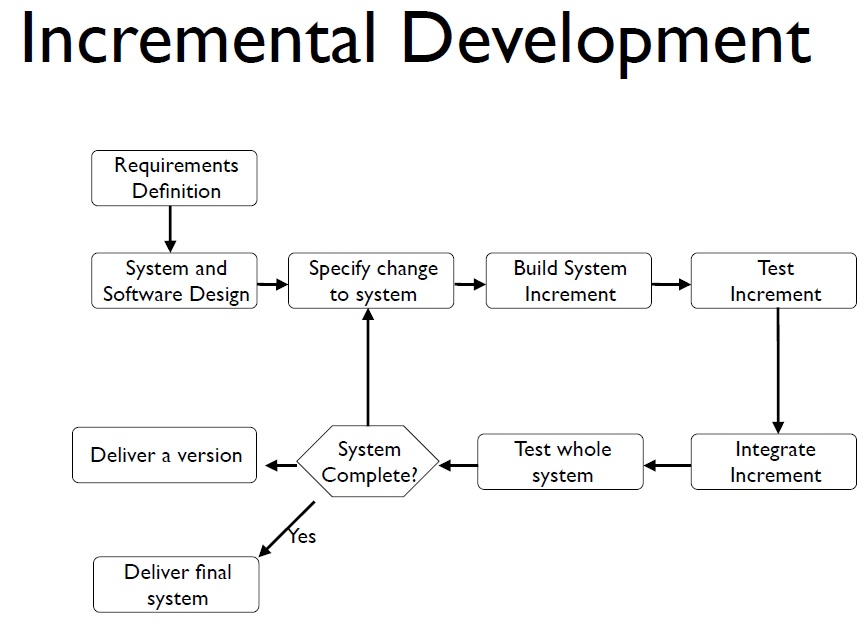
\includegraphics[scale=0.5]{incremental.jpg}\\

\section{Use Case}
This section will highlight the functional requirements that were defined in the
requirement pdf.

\subsection{Welcome Page}
Functional Requirements-
FR1 - Server-based Authentication
FR6 - Client Options
FR7 - Start-up of software in browser

\subsection{Main profile page}
Functional Requirements-
FR8 - Game Display In Browser
FR10 - Fight Notifications

\subsection{Friends Page}
Functional Requirements-
FR2 - Server Friends List
FR5 - Server-server communication
FR6 - Client Options
FR9 - Friend Matching
FR11- Friends Rich List

\subsection{Add Friends}
Functional Requirements-
FR5 - Server-server communication
FR6 - Client Options
FR9 - Friend Matching

\subsection{Breeding}
Functional Requirements-
FR3 - Server Monster List
FR5 - Server-server communication
FR6 - Client Options
FR8 - Game Display In Browser

\subsection{Breeding Results}
Functional Requirements-
FR5 - Server-server communication
FR6 - Client Options
FR8 - Game Display In Browser

\subsection{Battle Screen}
Functional Requirements-
FR4 - Server Monster mash management
FR5 - Server-server communication
FR6 - Client Options
FR8 - Game Display In Browser

\subsection{Battle Results Page}
Functional Requirements-
FR3 - Server Monster List
FR8 - Game display in browser
FR10 - Fight Notifications

\subsection{Help Page}

\subsection{Notifications Page}

\section{User Interface Design}

\subsection{Login Screen(fig2)}
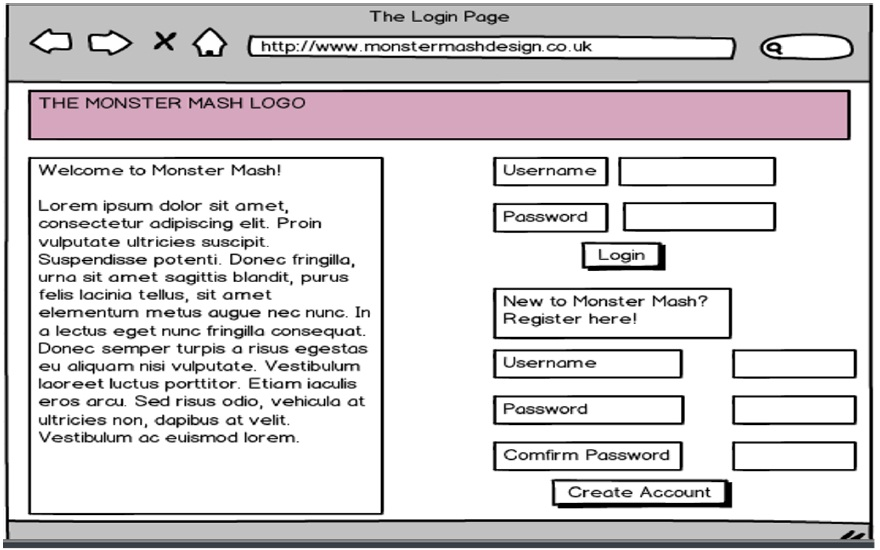
\includegraphics[scale=0.5]{loginPage.jpg}

\\
\\
This is the basic design of the page the user will first encounter when they want to
either create an account or log in if they already have an account. Both the Login
button and the Create Account button (if filled in correctly) will take the user to
their profile page. This is the only page in which the user is not signed into their
account.
Once logged in, the user will be directed to Figure 3.


\subsection{Profile page(fig3)}
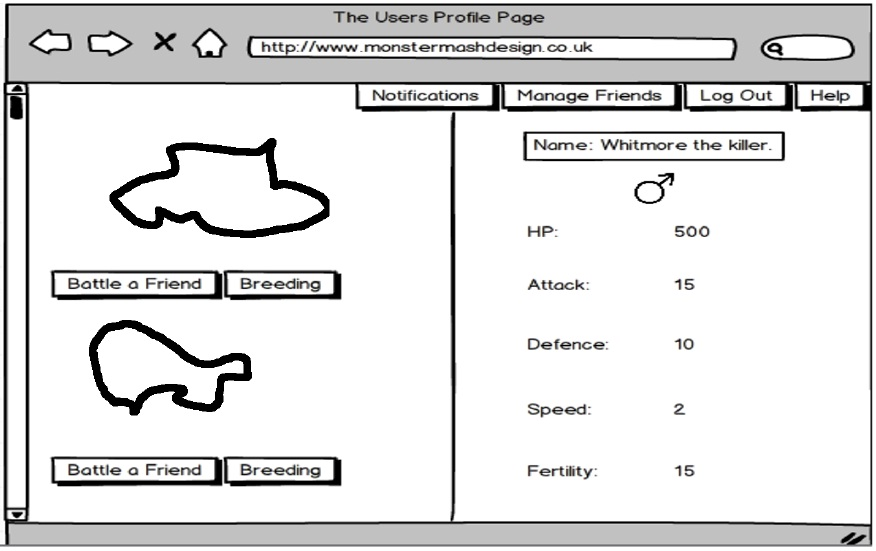
\includegraphics[scale=0.5]{userProfile.jpg}
\\
\\
This is the basic design for the profile page of our project, this will be the page
the login screen takes you each time you log in. It is from here, you (the user)
will be able to select each of your monsters to either battle or breed with a friends
monster. There are other features that are accessible from this page, such as the
Help page and the Manage Friends page, which can be seen in the top right corner of
the screen, however these are also accessible from other pages aside from the Profile
page, so we will just focus on the Breeding and Battle a Friend page.
On the right hand side of the page, the stats for the monster you have selected
will be shown, this will be done by clicking or possibly hovering over the monster
with the mouse.
You select which monster you want to breed by clicking on the corresponding
breeding button. Located underneath the monster you wish to select. Once you
have selected your monster you wish to breed. You are taken to figure 4.
\newpage


\subsection{Breeding Page(fig 4)}
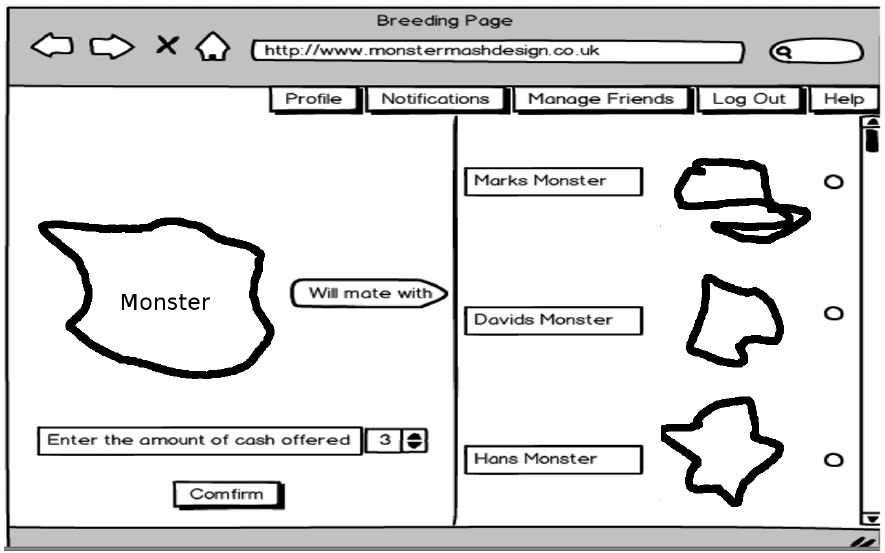
\includegraphics[scale=0.5]{breedingPage.jpg}

\\
\\
The monster that you selected for breeding from the previous page will be shown
on the left hand side of the screen, on the right hand side of the screen are all the
monsters that your friends own, the idea here being that you have to select one of
your friends monsters to breed with the monster you have, seeing that you are the
one who beneits from the breeding process (the one being requested to be bred with
does not gain a monster) the user must enter an amount of points, or cash into the
box located on the left hand side of the page (the one with the number 3 in it). It
is then up to the other player to either accept or reject this offer, if it is accepted,
the breeding takes place and the points are transacted from one users account into
the others. The player who initiated the breeding process then gains a monster.
Returning to Figure 3, if you want to select a monster to battle another friends
monster, as with breeding, simply select the corresponding button underneath the
monster of your choice, you will then be taken to Figure 5.
\newpage

\subsection{Battle Selection Screen(fig 5)}
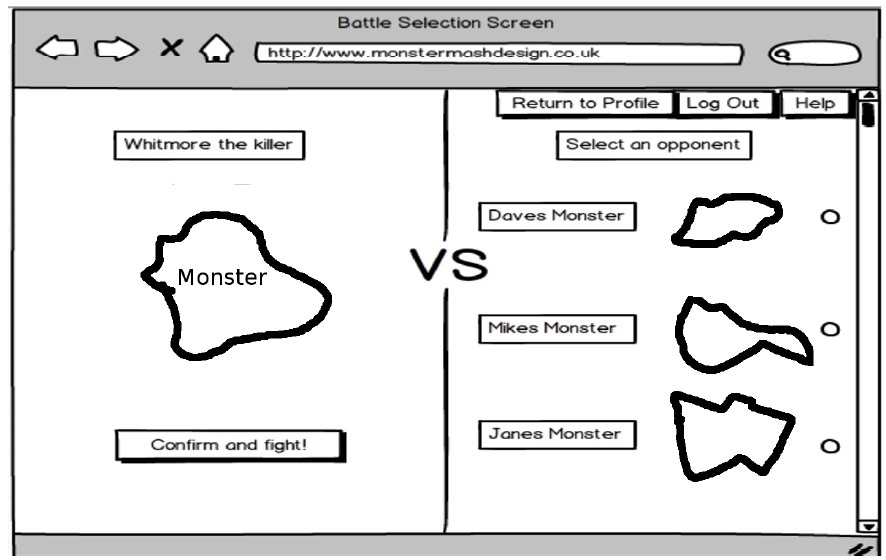
\includegraphics[scale=0.5]{battleSelection.jpg}

\\
\\
Similar to the breeding page, this requires the user to select one of their friends
monsters to challenge, once they have selected, the user simply presses the confirm
and fight button, and the request is sent.
Both pending battle and breeding requests can be viewed in the Manage Friends
page. Incoming requests will appear on your notifications.

\subsection{Battle Page(fig 6)}
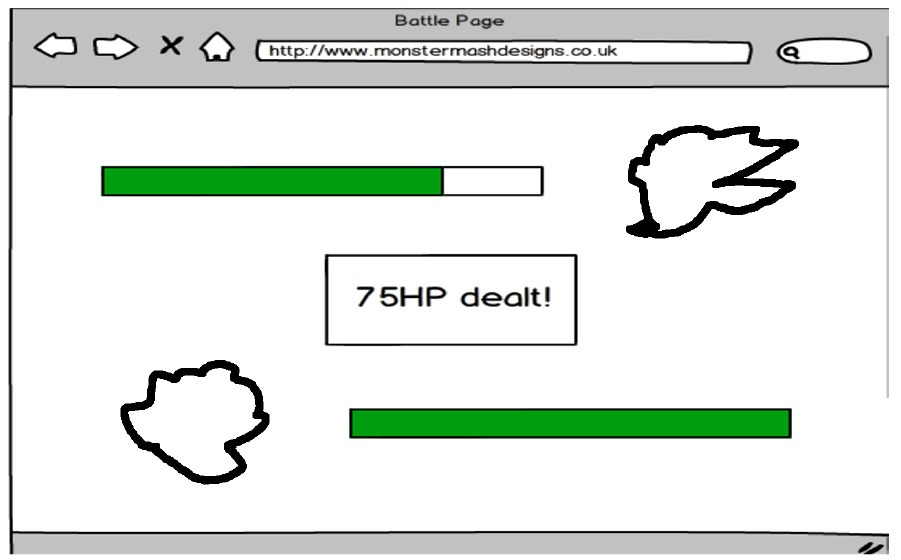
\includegraphics[scale=0.5]{battle.jpg}
\\
\\
It should be noted that this page will only be viewed by the user accepting the battle
request. Once the user has accepted a battle request off their friend, they will be
redirected to this page.
This is an example of a battle taking place between two monsters. The user (so
the one who accepted the battle request) can watch the battle unfold. The text
in the middle constantly updates, telling the user how much damage each monster
deals to each other. The green bar next to each of the monsters is their health bar,
this gradually decreases as the battle progresses. The first monster to lose all of its
life it declared the loser. After the battle, the user is directed back to the Profile
page (Figure 3), the other user that wasnt present for the fight receives a message
in their notifications telling them how the fight unfolded.
Moving back to Figure 3, if the Help button, located in the top right hand corner
is selected, Figure 7 should appear.

\subsection{The Help Page(fig 7)}
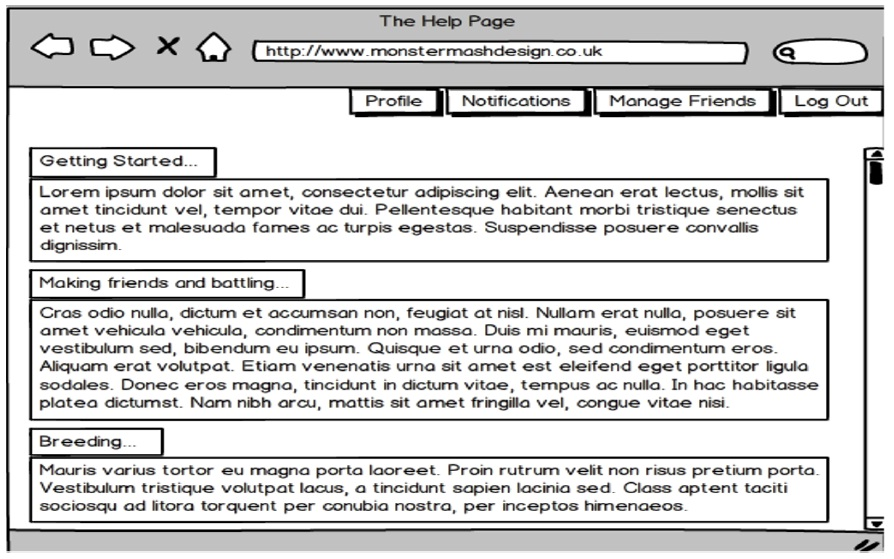
\includegraphics[scale=0.5]{help.jpg}
\\
\\
A simple page in design and implementation. This page will tell the user all they
need to know about how to user the application, including things such as how to
battle, how to breed and how to add friends.

\subsection{Friend Management Page(fig 8)}
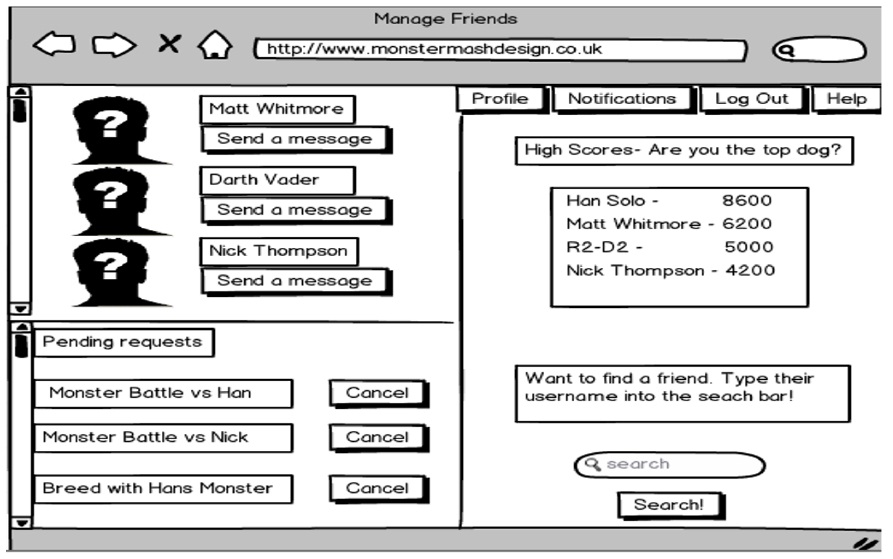
\includegraphics[scale=0.5]{manageFriends.jpg}
\\
\\
The Manage Friends page can be accessed from most of the web pages, the button
that directs to it is located in the top right hand corner of the screen.
The Manage Friends page holds many functions. From here you are able to cancel
pending requests to either battle or breed with another friends monster, send per-
sonal messages to your friends, and new friends to your list and also check who has
the top score overall out of all your friends.
To log out of Monster Mash, simple click the Log Out button which is found on
most of the pages to the top right hand corner. This will take you to back to Figure
1.
\section{Gantt chart}
This is the Gantt chart that is used for assigning tasks and a time period that those
tasks should be finished by. The image below is merely an example as the actual
Gantt chart is constantly changing. Can be seen online at
Gantt Chart

\section{Risk Assessment}
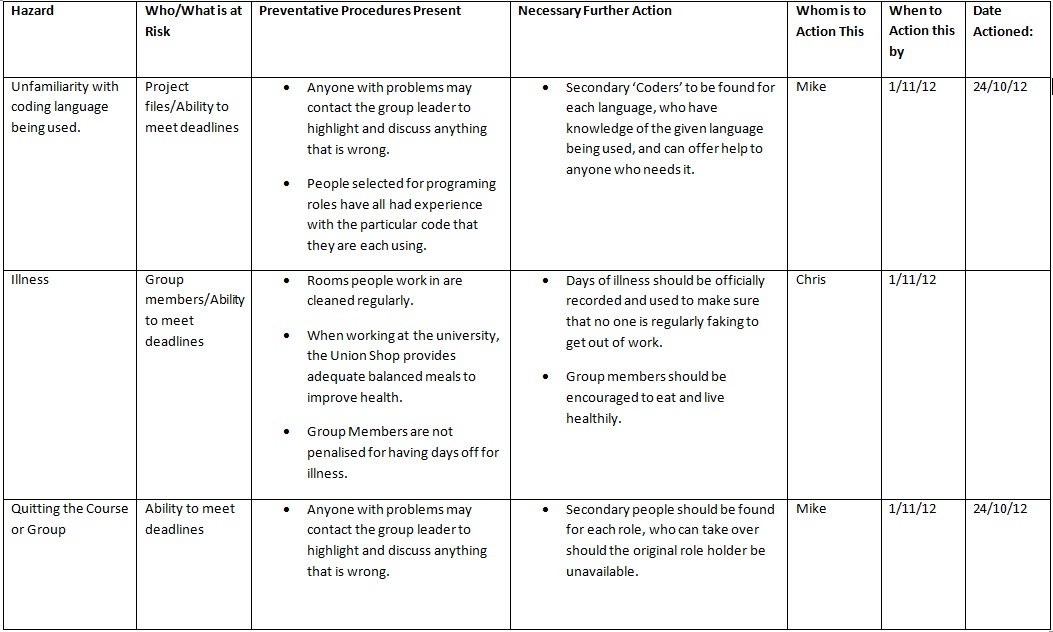
\includegraphics[scale=0.6]{risk1.jpg}\\
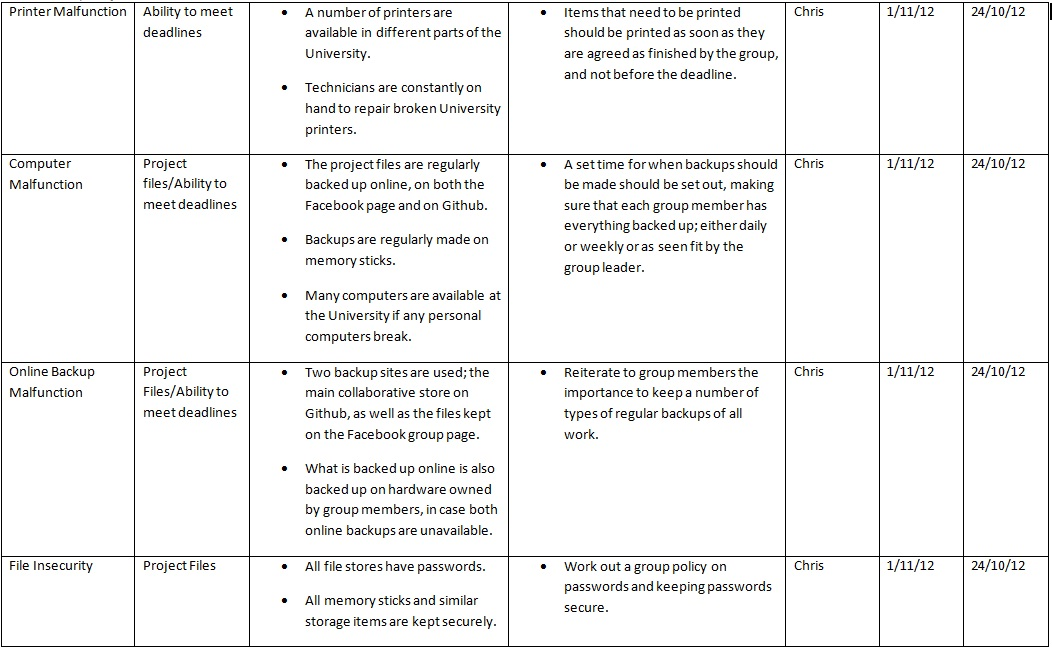
\includegraphics[scale=0.6]{risk2.jpg}\\
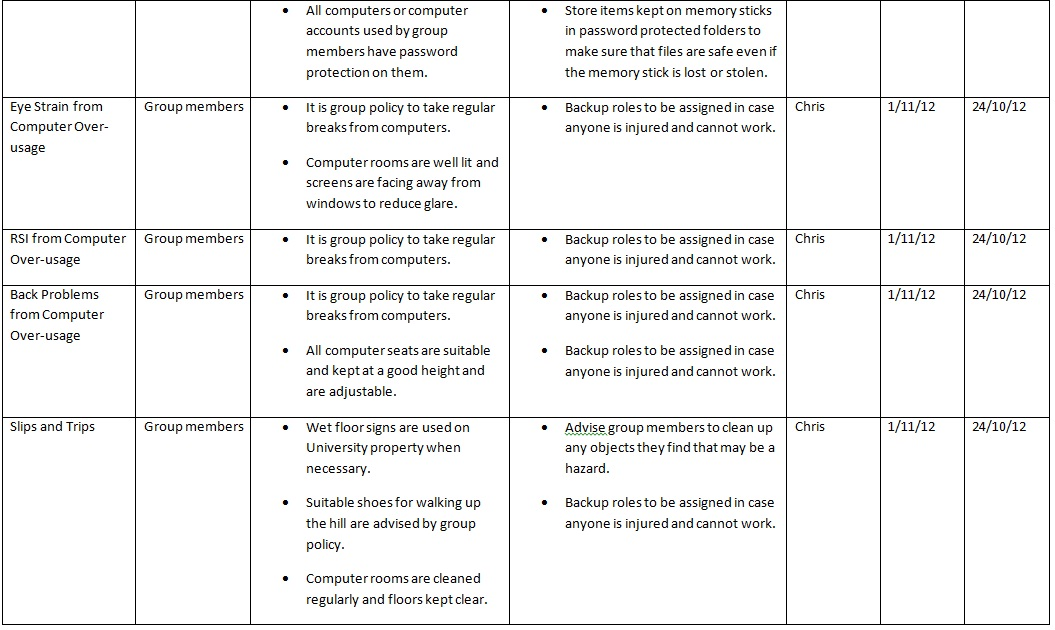
\includegraphics[scale=0.6]{risk3.jpg}\\
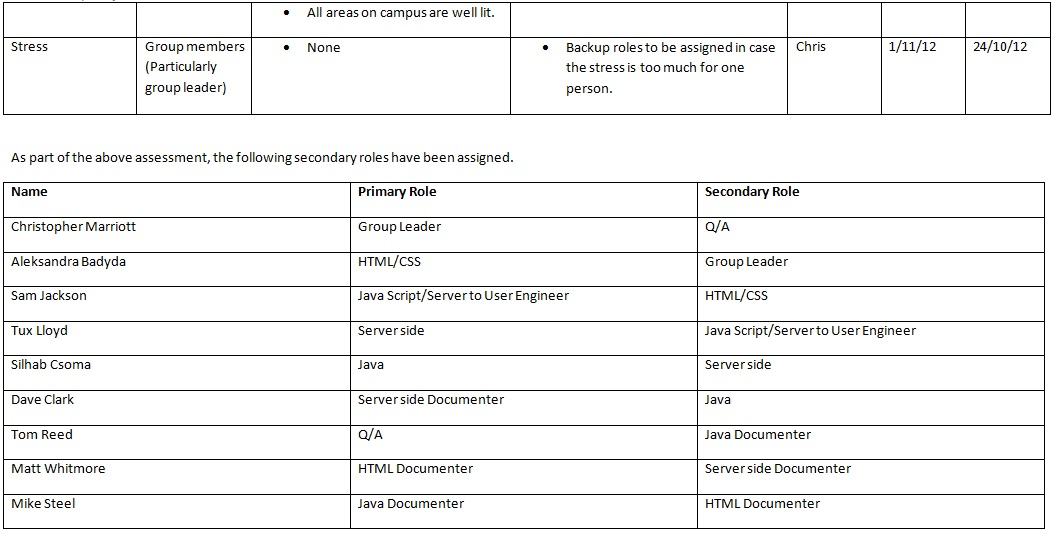
\includegraphics[scale=0.6]{risk4.jpg}\\
\clearpage
\addcontentsline{toc}{section}{REFERENCES}
\begin{thebibliography}{5}
\bibitem{} \emph{N/A}
\end{thebibliography}
\clearpage
\addcontentsline{toc}{section}{DOCUMENT HISTORY}
\section*{DOCUMENT HISTORY}
\begin{tabular}{|l | l | l | l | l |}
\hline
Version & CCF No. & Date & Changes made to Document & Changed by \\
\hline
1.0 & N/A & 2012-10-31 & Initial creation & CPM4 \\
\hline
1.1 & N/A & 2012-11-2 & Added information from Mike & CPM4 \\
\hline
1.2 & N/A & 2012-12-5 & Updated config ref and added other documents & CPM4 \\
\hline
1.3 & N/A & 2012-12-6 & Added missing data and fixed few mistakes & CPM4 \\
\hline
\end{tabular}
\label{thelastpage}
\end{document}

=======
\documentclass{project}
\usepackage[pdfauthor={C. P. Marriott},pdftitle={Software Engineering Group Project, Project Plan},pdftex]{hyperref}
\usepackage[pdftex]{graphicx}
\usepackage{pdfpages}
\hypersetup{colorlinks=false,pdfborder={0 0 0}}
\begin{document}
\title{Software Development Life cycle}
\subtitle{Project Plan}
\author{Tom Reed, Matt Whitmore, Dave Clark, Silhab Csoma, Mike Steel, Chris 'Tux' Lloyd, Aleksandra Badyda, Samuel Jackson, Chris Marriott}
\shorttitle{Project Plan}
\version{1.3}
\status{draft}
\date{2012-12-5}
\configref{SE.17.DS.01}
\maketitle
\tableofcontents
\newpage
\section{Introduction}
\subsection{Purpose of this Document}
This is the user interface specification. This document is intended to show how the system will look and feel. It will also show the risk assessment and the Gantt chart.
\subsection{Scope}
This document will show how the user will be able to interact with the system
through use case diagrams. How the system will look through user interface design.
It will also list the risks that could possibly arise and what people in the groups
primary and secondary roles are. This will be shown in the risk assessment. There
will also be a example Gantt chart that will list people in the group, their task and
time frame for which it is intended to be completed.

\subsection{Objectives}
The objective of this document is to design the interface and usability of the system
for the monster mash game.
The areas covered by this plan are:
\\
Start bullet points
\begin{itemize}
	\item Overview of system
	\item Use Cases
	\item User Interface mock ups
	\item Gantt Chart
	\item Risk Analysis
\end{itemize}

\section{Overview}
This project requires the group to be able to design and create a web based applica-
tion that allows the users to socially interact with one another. Monster Mash (The
name of the social web application) will allow the user to create an online profile and
once this is completed, the application will give each new user their own monster,
of which they can use to challenge other users of the application to a battle, and
depending on the outcome (win or lose) will award you with points and will alter
the statistics of your monster.
To commence a battle with another user, its required that they are both "Friends"
with one other on the web application, like many other social networking sites, this
will be done by one user sending a friend request, and the other either accepting or
rejecting.
Aside from battling each others monsters, the game should be able to include other
features such as breeding, so that users can create stronger monsters, and also a
high scores page, on which friends can check to see who has the best overall score
out of each of them.
\section{Deployment}
\subsection{Overview}
We have decided to use a small enterprise style system, which will be hosted on
Chris Lloyds VPS (virtual private server). While this would normally not be hosted
on a single server (due to security), it does allow almost all of the benets such as it
being live(non-local), 99.9% uptime and self-managed hosting. It also gives us some
experience with how to deal with real world solutions that we may come across in
our future lines of work.

\subsection{Hosting}
The hosting has been sorted by Chris Lloyd; he has allowed the group to use his
VPS which he has installed Apache http server, MySQL database and a tomcat.
Chris Lloyd has also purchased the domain monstermashgame.co.uk to which he
has added an A-record to the VPSs IP.

\subsection{Apache HTTP}
Apache is used to handle http requests; this will mainly involve sending html pages
that has been requested. Apache is the worlds most widely used http server and is
used as the standard in industry.

\subsection{MySQL}
MySQL, while not being used at the higher end of the corporate market (held by
Oracle), it does allow us to use an enterprise like database system, as it is quite
commonly used for small to medium sized business and is often used on small scale
web hosting.
\subsection{TomCat}
Tomcat as a project, is developed by the Apache foundation. Tomcat is widely
deployed as a java application server, all though through the various configurations
it can be used to make a mass distributed java cluster. This is to say that it is
possible to run a single java application across a distributed processing cluster.
\subsection{server Side Conclusion}
While there is other software out there that may do a better job, we found that by
sticking to the widely used software, implementation and application, we would find
a good, well rounded base knowledge in the area of server side web applications.
\section{Methodology}
Although the structure of the hand in documents leads us to waterfall, we shall aim
to do incremental within this.
The advantages are:
\\
Start bullet points
\begin{itemize}
	\item Easier management
	\item Can get user feedback earlier
	\item Can avoid crises by be alerted to problems earlier
	\item Can respond easier to changing user requirements
	\item Earlier exchange of functionlaity
\end{itemize}

The disadvantages are:
\begin{itemize}
	\item Can be harder to manage, with more steps and crucial decencies and overall
progress monitoring
	\item Version and configuration control is crucial and can be complex
\end{itemize}

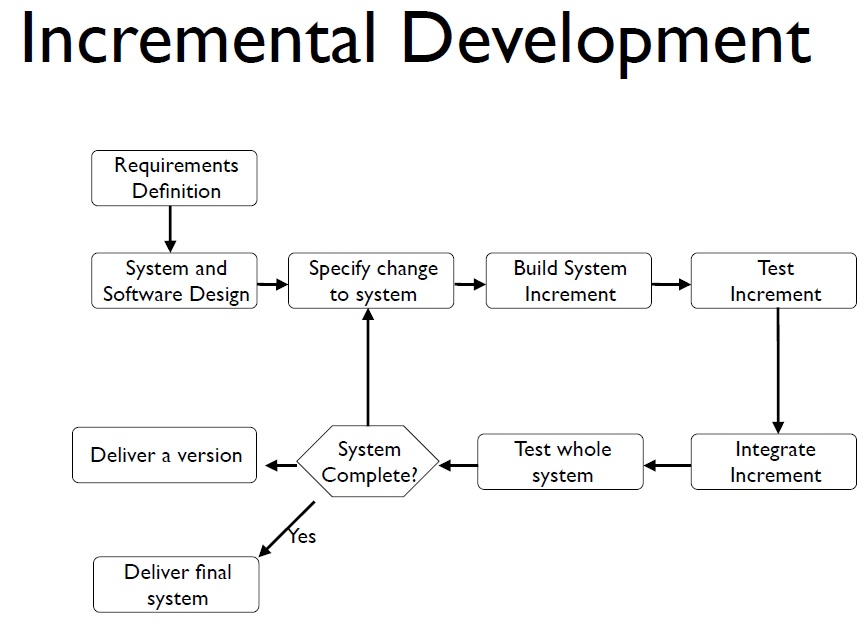
\includegraphics[scale=0.5]{incremental.jpg}\\

\section{Use Case}
This section will highlight the functional requirements that were defined in the
requirement pdf.

\subsection{Welcome Page}
Functional Requirements-
FR1 - Server-based Authentication
FR6 - Client Options
FR7 - Start-up of software in browser

\subsection{Main profile page}
Functional Requirements-
FR8 - Game Display In Browser
FR10 - Fight Notifications

\subsection{Friends Page}
Functional Requirements-
FR2 - Server Friends List
FR5 - Server-server communication
FR6 - Client Options
FR9 - Friend Matching
FR11- Friends Rich List

\subsection{Add Friends}
Functional Requirements-
FR5 - Server-server communication
FR6 - Client Options
FR9 - Friend Matching

\subsection{Breeding}
Functional Requirements-
FR3 - Server Monster List
FR5 - Server-server communication
FR6 - Client Options
FR8 - Game Display In Browser

\subsection{Breeding Results}
Functional Requirements-
FR5 - Server-server communication
FR6 - Client Options
FR8 - Game Display In Browser

\subsection{Battle Screen}
Functional Requirements-
FR4 - Server Monster mash management
FR5 - Server-server communication
FR6 - Client Options
FR8 - Game Display In Browser

\subsection{Battle Results Page}
Functional Requirements-
FR3 - Server Monster List
FR8 - Game display in browser
FR10 - Fight Notifications

\subsection{Help Page}

\subsection{Notifications Page}

\section{User Interface Design}
\subsection{Login Screen(fig2)}
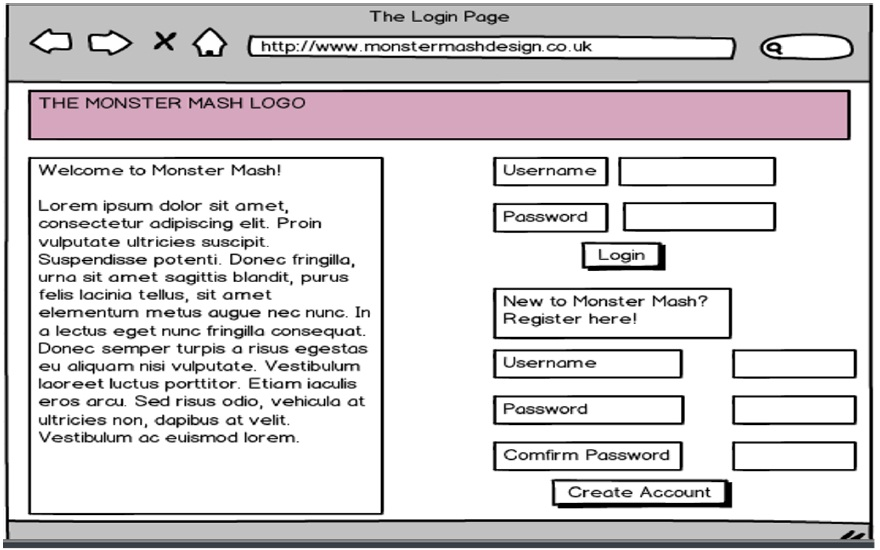
\includegraphics[scale=0.5]{loginPage.jpg}\\
This is the basic design of the page the user will first encounter when they want to
either create an account or log in if they already have an account. Both the Login
button and the Create Account button (if filled in correctly) will take the user to
their profile page. This is the only page in which the user is not signed into their
account.
Once logged in, the user will be directed to Figure 3.

\subsection{Profile page(fig3)}
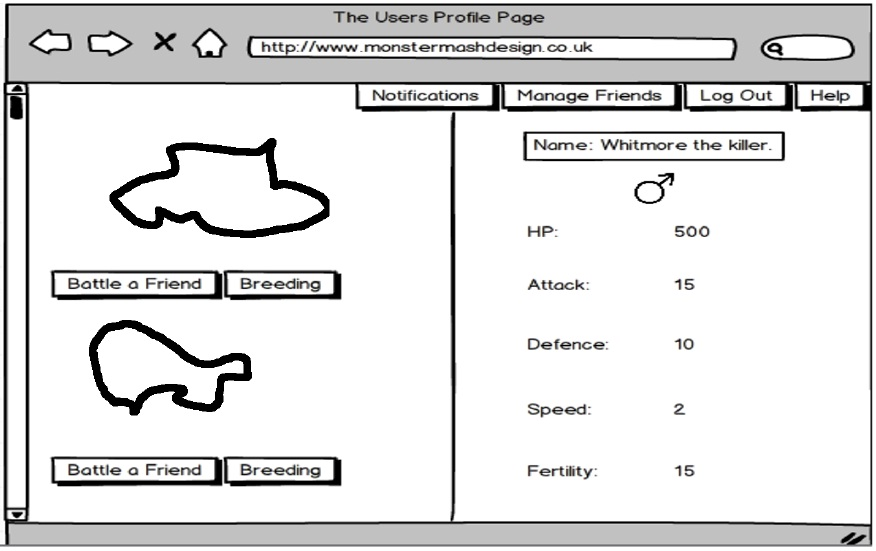
\includegraphics[scale=0.5]{userProfile.jpg}\\
This is the basic design for the profile page of our project, this will be the page
the login screen takes you each time you log in. It is from here, you (the user)
will be able to select each of your monsters to either battle or breed with a friends
monster. There are other features that are accessible from this page, such as the
Help page and the Manage Friends page, which can be seen in the top right corner of
the screen, however these are also accessible from other pages aside from the Prole
page, so we will just focus on the Breeding and Battle a Friend page.
On the right hand side of the page, the stats for the monster you have selected
will be shown, this will be done by clicking or possibly hovering over the monster
with the mouse.
You select which monster you want to breed by clicking on the corresponding
breeding button. Located underneath the monster you wish to select. Once you
have selected your monster you wish to breed. You are taken to figure 4.

\subsection{Breeding Page(fig 4)}
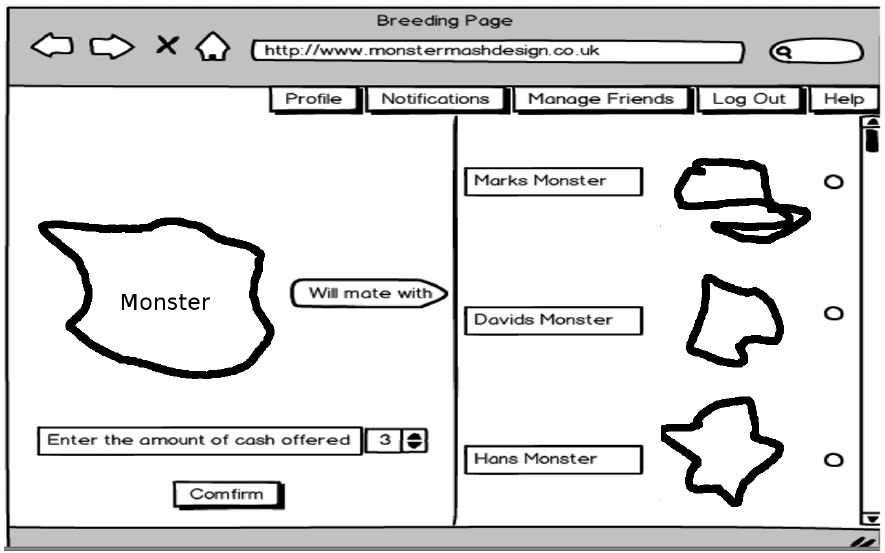
\includegraphics[scale=0.5]{breedingPage.jpg}\\
The monster that you selected for breeding from the previous page will be shown
on the left hand side of the screen, on the right hand side of the screen are all the
monsters that your friends own, the idea here being that you have to select one of
your friends monsters to breed with the monster you have, seeing that you are the
one who benets from the breeding process (the one being requested to be bred with
does not gain a monster) the user must enter an amount of points, or cash into the
box located on the left hand side of the page (the one with the number 3 in it). It
is then up to the other player to either accept or reject this oer, if it is accepted,
the breeding takes place and the points are transacted from one users account into
the others. The player who initiated the breeding process then gains a monster.
Returning to Figure 3, if you want to select a monster to battle another friends
monster, as with breeding, simply select the corresponding button underneath the
monster of your choice, you will then be taken to Figure 5.

\subsection{Battle Selection Screen(fig 5)}
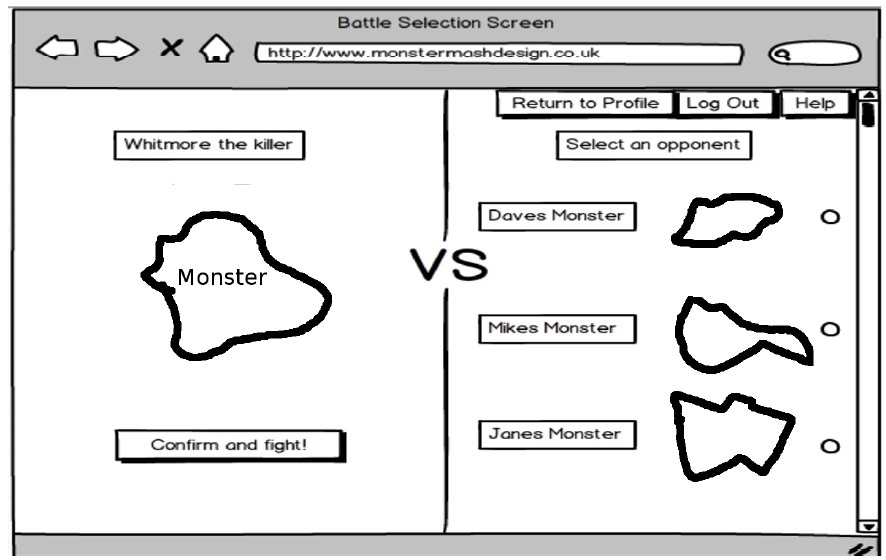
\includegraphics[scale=0.5]{battleSelection.jpg}\\
Similar to the breeding page, this requires the user to select one of their friends
monsters to challenge, once they have selected, the user simply presses the conrm
and fight button, and the request is sent.
Both pending battle and breeding requests can be viewed in the Manage Friends
page. Incoming requests will appear on your notifications.

\subsection{Battle Page(fig 6)}
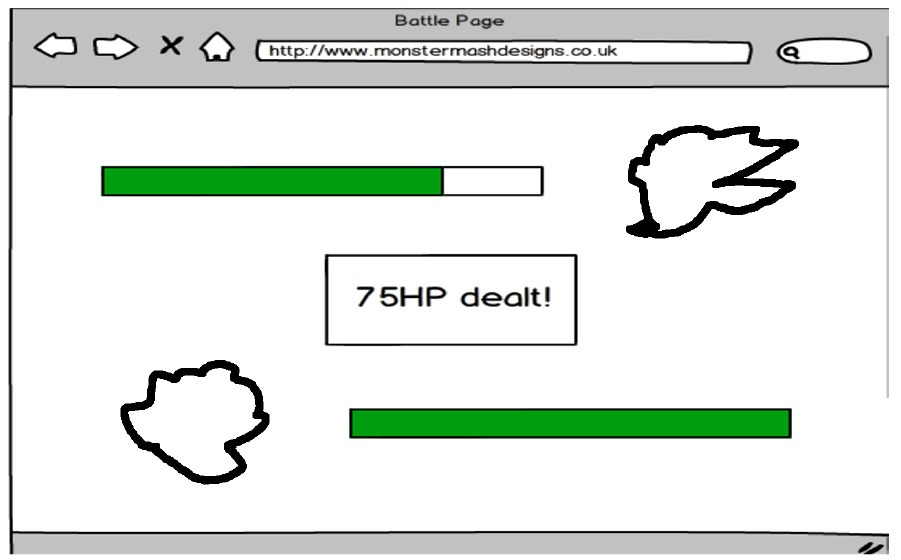
\includegraphics[scale=0.5]{battle.jpg}\\
It should be noted that this page will only be viewed by the user accepting the battle
request. Once the user has accepted a battle request o their friend, they will be
redirected to this page.
This is an example of a battle taking place between two monsters. The user (so
the one who accepted the battle request) can watch the battle unfold. The text
in the middle constantly updates, telling the user how much damage each monster
deals to each other. The green bar next to each of the monsters is their health bar,
this gradually decreases as the battle progresses. The rst monster to lose all of its
life it declared the loser. After the battle, the user is directed back to the Prole
page (Figure 3), the other user that wasnt present for the ght receives a message
in their notifications telling them how the fight unfolded.
Moving back to Figure 3, if the Help button, located in the top right hand corner
is selected, Figure 7 should appear.

\subsection{The Help Page(fig 7)}
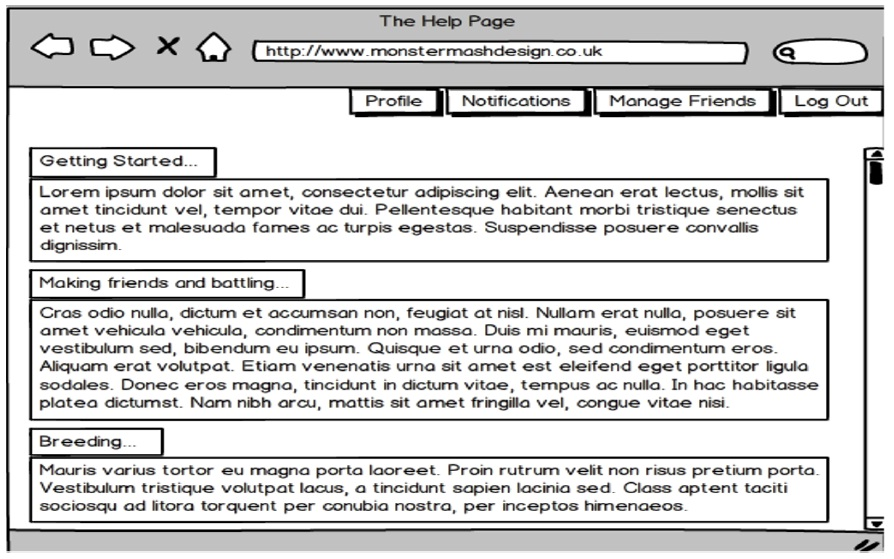
\includegraphics[scale=0.5]{help.jpg}\\
A simple page in design and implementation. This page will tell the user all they
need to know about how to user the application, including things such as how to
battle, how to breed and how to add friends.

\subsection{Friend Management Page(fig 8)}
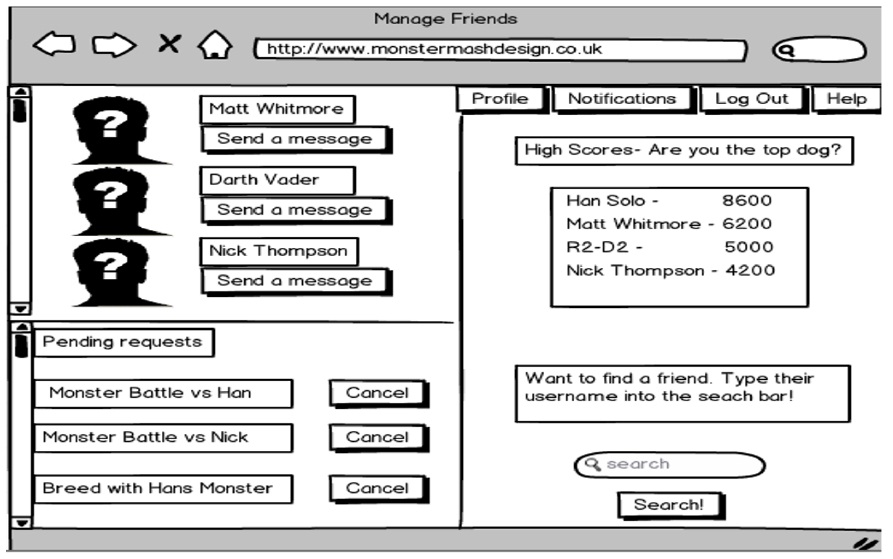
\includegraphics[scale=0.5]{manageFriends.jpg}\\
The Manage Friends page can be accessed from most of the web pages, the button
that directs to it is located in the top right hand corner of the screen.
The Manage Friends page holds many functions. From here you are able to cancel
pending requests to either battle or breed with another friends monster, send per-
sonal messages to your friends, and new friends to your list and also check who has
the top score overall out of all your friends.
To log out of Monster Mash, simple click the Log Out button which is found on
most of the pages to the top right hand corner. This will take you to back to Figure
1.
\section{Gantt chart}
This is the Gantt chart that is used for assigning tasks and a time period that those
tasks should be finished by. The image below is merely an example as the actual
Gantt chart is constantly changing. Can be seen online at
Gantt Chart

\section{Risk Assessment}
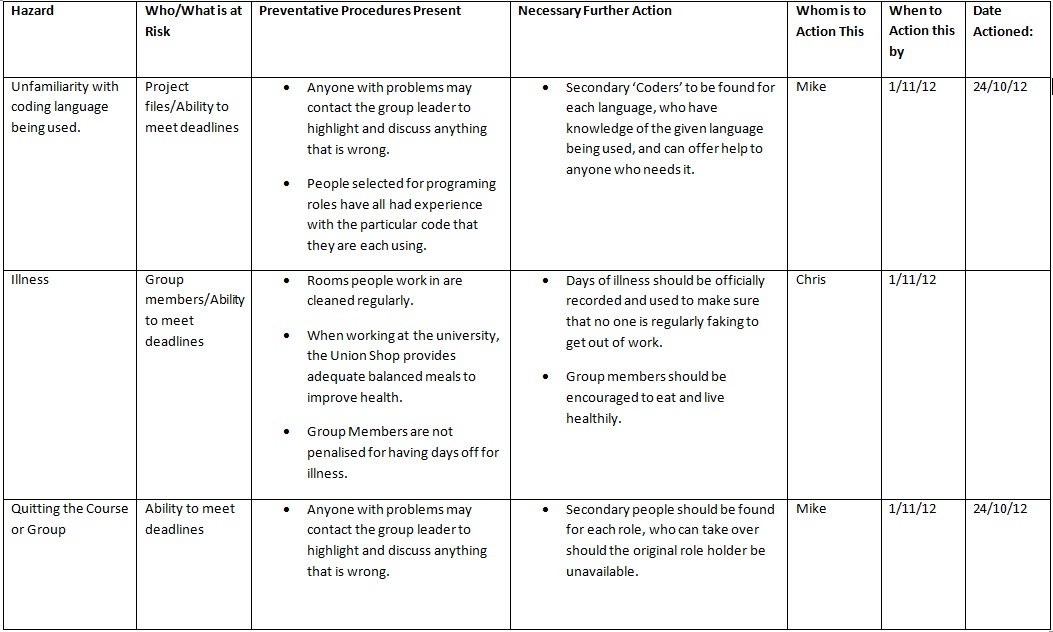
\includegraphics[scale=0.6]{risk1.jpg}\\
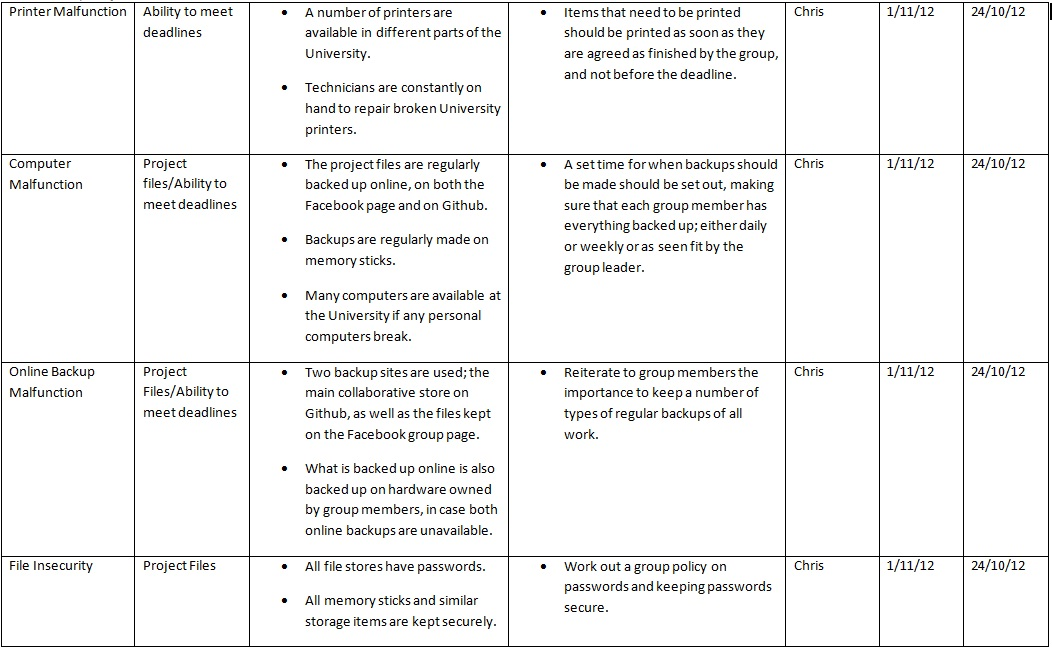
\includegraphics[scale=0.6]{risk2.jpg}\\
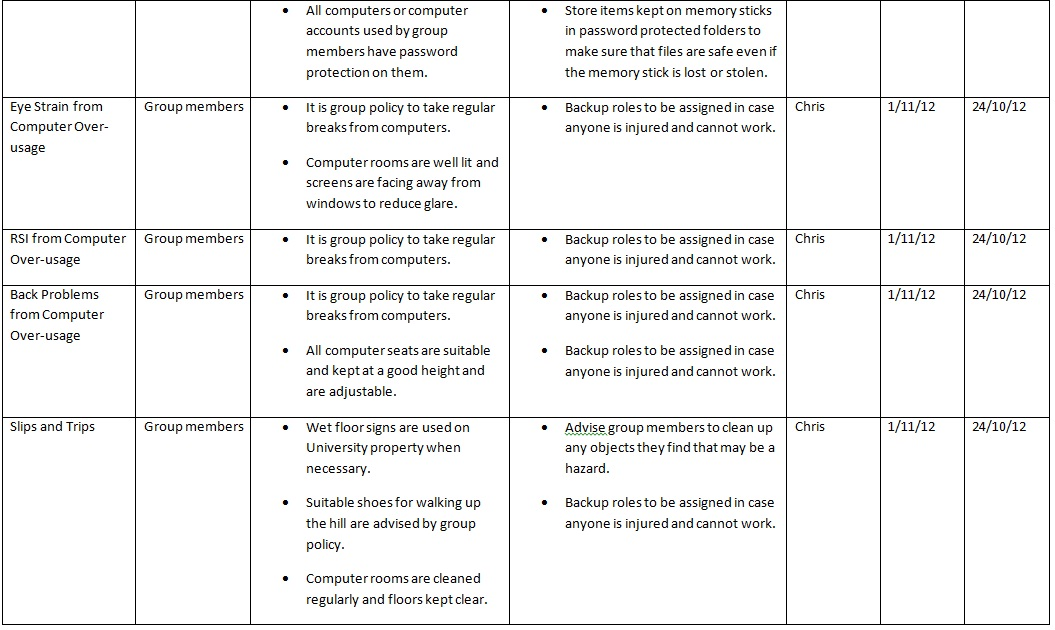
\includegraphics[scale=0.6]{risk3.jpg}\\
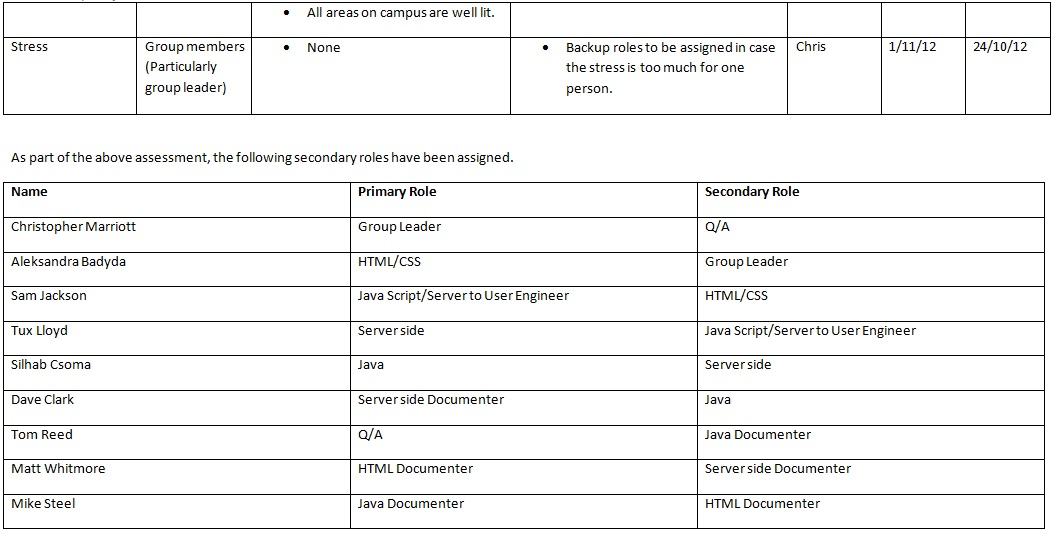
\includegraphics[scale=0.6]{risk4.jpg}\\
\clearpage
\addcontentsline{toc}{section}{REFERENCES}
\begin{thebibliography}{5}
\bibitem{} \emph{N/A}
\end{thebibliography}
\clearpage
\addcontentsline{toc}{section}{DOCUMENT HISTORY}
\section*{DOCUMENT HISTORY}
\begin{tabular}{|l | l | l | l | l |}
\hline
Version & CCF No. & Date & Changes made to Document & Changed by \\
\hline
1.0 & N/A & 2012-10-31 & Initial creation & CPM4 \\
\hline
1.1 & N/A & 2012-11-2 & Added information from Mike & CPM4 \\
\hline
1.2 & N/A & 2012-12-5 & Updated config ref and added other documents & CPM4 \\
\hline
1.3 & N/A & 2012-12-6 & Added missing data and fixed few mistakes & CPM4 \\
\hline
\end{tabular}
\label{thelastpage}
\end{document}

>>>>>>> c0c3b16f1f5888737f0b30cb0cee2b0dc76e0dce:N17/docs/Project Plan/projectplan.tex
